\vspace{-0.1in}
\begin{figure}[h]
    \centering
    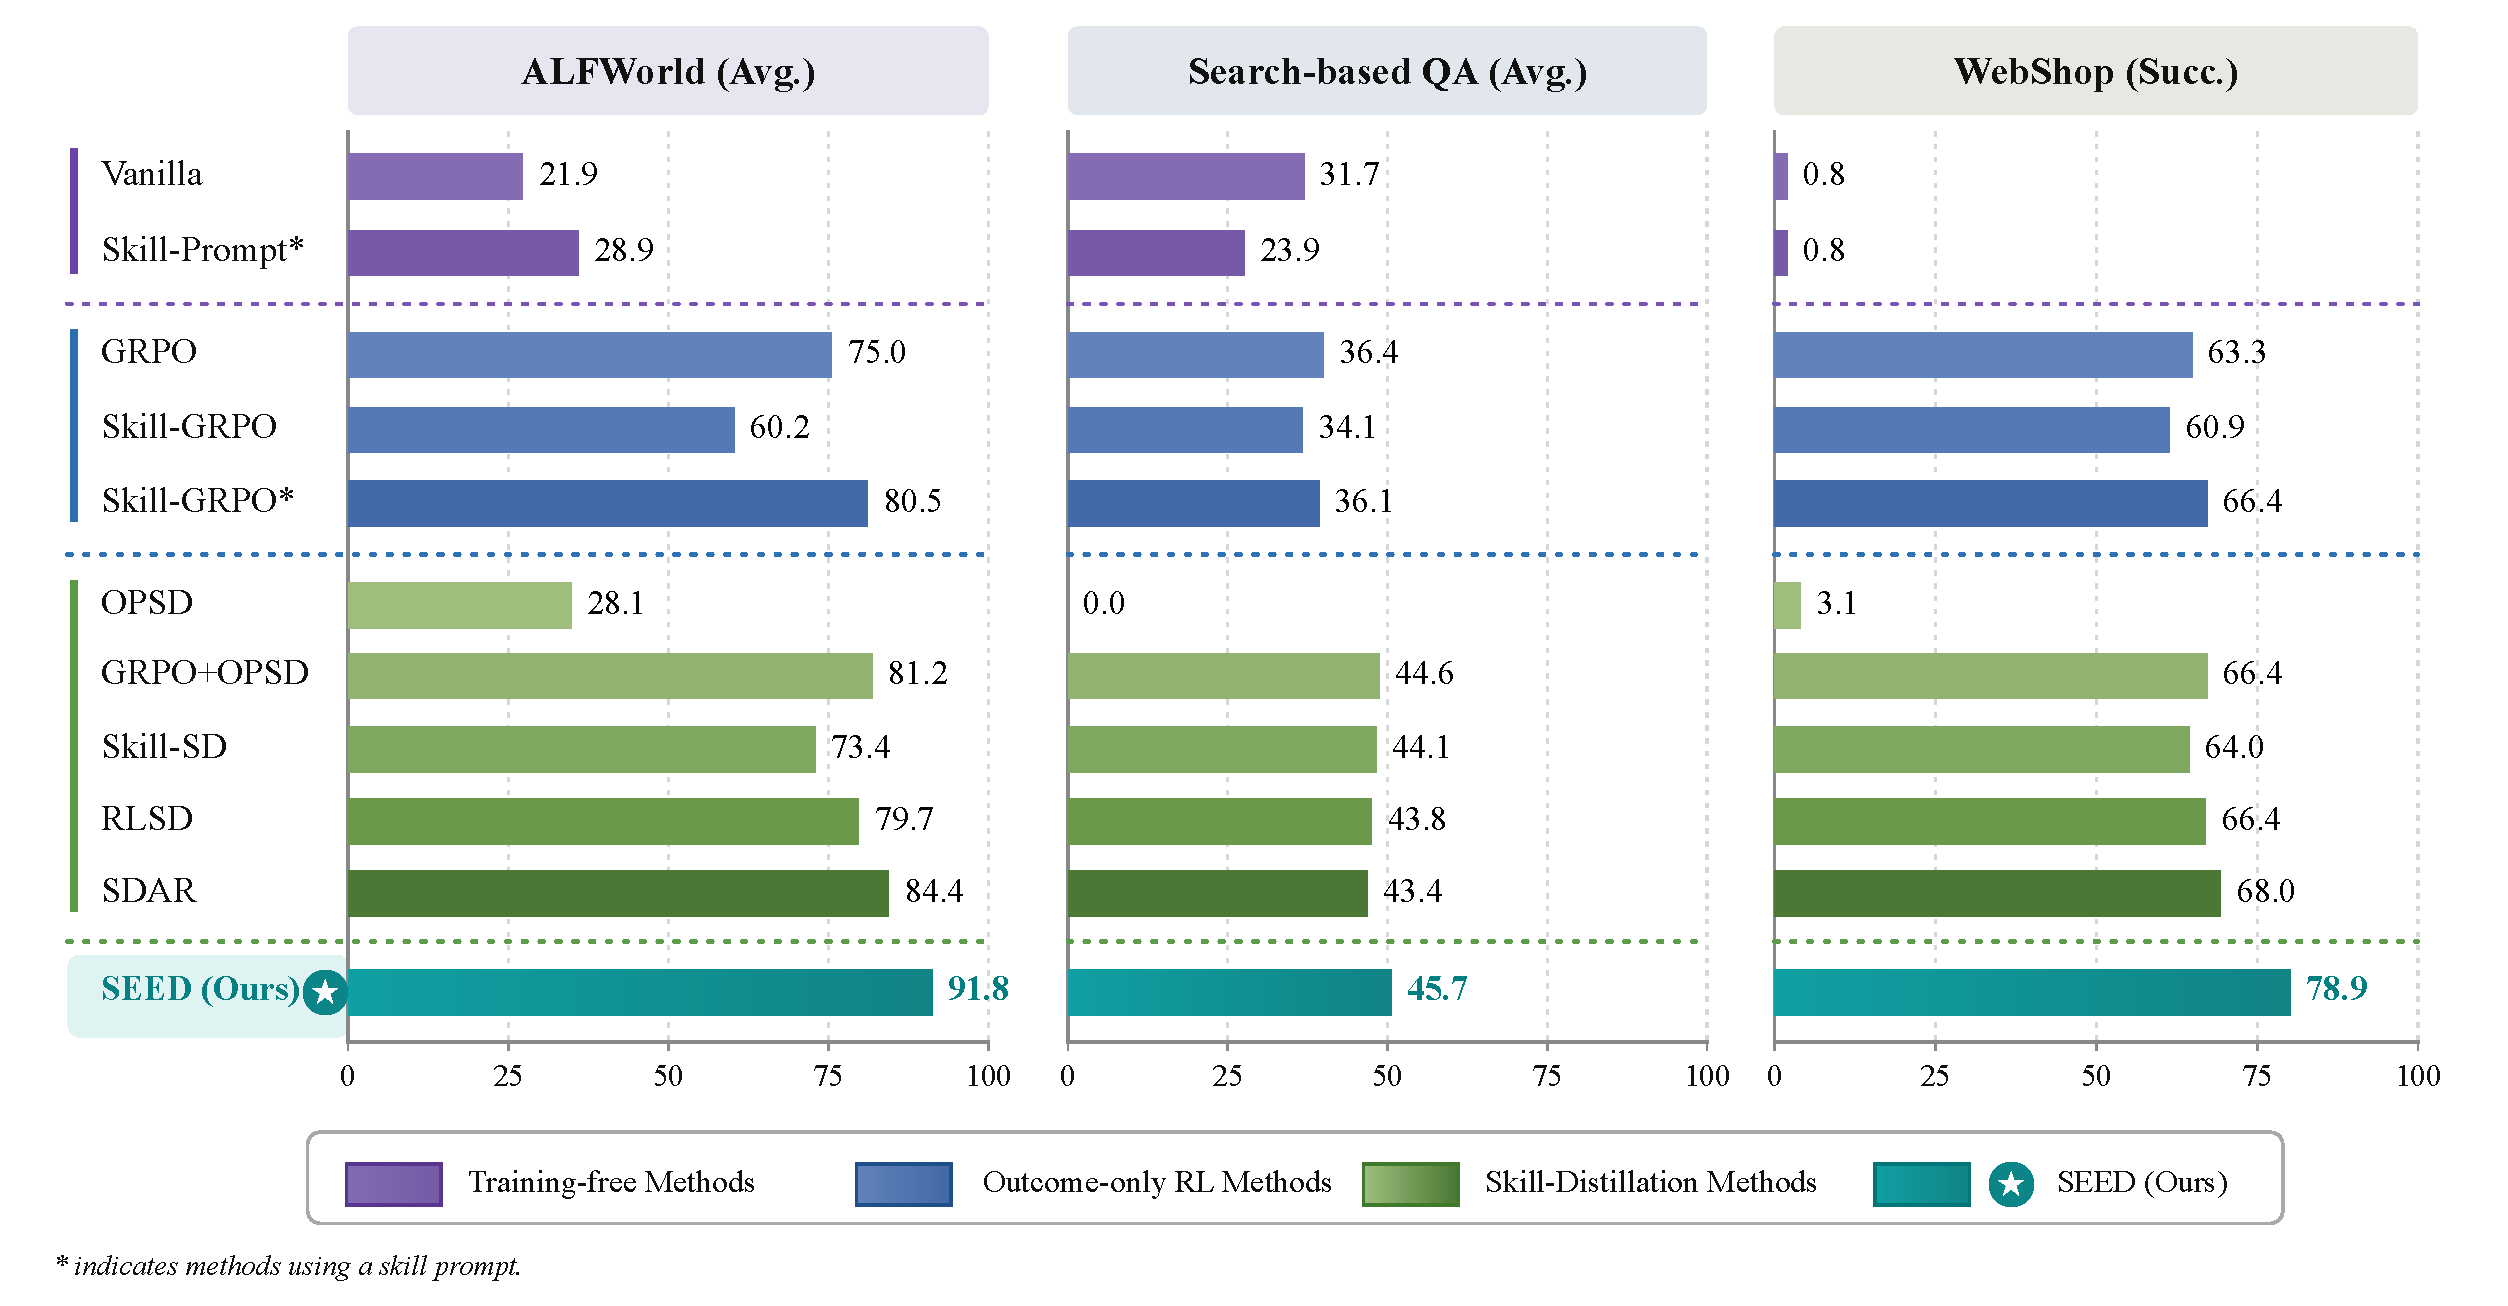
\includegraphics[width=0.99\linewidth]{figures/overall_performance_comparison_3b.pdf}
    \caption{
        \textbf{Overall performance overview.}
        Compared with powerful baseline methods, \textsc{Seed} achieves the strongest average performance across three representative agentic benchmarks.
    }
    \label{fig:overall_performance}
\end{figure}

\section{Introduction}\label{sec1_intro}
Recent large language model (LLM) systems are moving beyond single-turn response generation toward multi-turn agentic interaction, where a model repeatedly reasons, acts, uses tools, and incorporates feedback from its environment~\citep{liu2023agentbench,schick2023toolformer,patil2024gorilla,luo2025large,xi2025rise,wu2026atlas,xu2026odysseyarena}. Such settings require an agent to make sequential decisions whose consequences may only become visible after many interaction steps. The model must learn when to gather information, when to call a tool, how to interpret feedback, and how to revise a plan after partial progress or failure. Reinforcement learning (RL) has therefore become an important post-training paradigm for LLM-based agents, since it directly optimizes policies against task-level feedback from environments, simulators, or verifiers~\citep{shao2024deepseekmath,wang2025ragen,luo2025agentlightning,wu2026spark}.

Despite this progress, outcome-based agentic RL provides only coarse supervision. In long-horizon environments, rewards are often sparse, delayed, and assigned at the trajectory level: they indicate whether an episode succeeds but not which intermediate observations, actions, or tool calls should be reinforced or corrected~\citep{andrychowicz2017hindsight,arjona2019rudder,uesato2022solving,lightman2024lets}. This leaves a supervision gap between episode-level outcomes and token-level policy learning. A failed trajectory may contain useful partial behaviors but fail because of a few local mistakes, whereas a successful trajectory may contain reusable strategies that the scalar reward never identifies. As a result, outcome-only optimization provides limited guidance for fine-grained, decision-level credit assignment over long interaction histories.

A key observation is that completed trajectories reveal hindsight unavailable during online decision making. Once an episode terminates, the full interaction history reveals which subgoals were achieved, where the agent deviated from an effective strategy, which observations were decisive, and which behavioral patterns may transfer to future attempts. This view is related to hindsight learning in RL, where completed experience can be reinterpreted to improve learning under sparse feedback~\citep{andrychowicz2017hindsight}, and to language-agent methods based on verbal reflection, episodic memory, or experience summaries~\citep{shinn2023reflexion,zhao2024expel,wang2023voyager,madaan2023selfrefine}. However, many such methods treat hindsight as static experience, inference-time context, or retrieved memory. For practical agentic RL, hindsight supervision should not remain fixed: as the policy improves and encounters new states, strategies, and failure modes, the hindsight extracted from its trajectories must adapt to its current behavior~\citep{andrychowicz2017hindsight,zhang2026the}. Our goal is therefore to convert policy-generated hindsight into parametric supervision, enabling the policy to internalize reusable behavioral guidance without external memory or additional deployment-time prompts.

On-policy distillation (OPD) offers a natural mechanism for converting hindsight information into decision-level learning signals. Classical knowledge distillation transfers teacher behavior into a student through token- or sequence-level supervision~\citep{hinton2015distilling,kim2016sequence}, while on-policy variants reduce distribution mismatch by supervising outputs sampled from the student policy itself~\citep{ross2011reduction,agarwal2024onpolicy}. Recent on-policy self-distillation methods further avoid a separate external teacher by comparing the same model under different contexts, such as privileged reasoning traces or feedback-conditioned prompts~\citep{zhao2026selfdistilledreasoner,hubotter2026sdpo}. Related agentic methods have explored skill- or feedback-conditioned distillation for multi-turn interaction and tool use~\citep{wang2026skillsd,lu2026sdar,zhong2026sod,ko2026reopold,yang2026opid}. Together, these advances point to three requirements for effective hindsight supervision in agentic RL.

First, the supervision should be \emph{on-policy}, because useful corrections depend on the states, actions, and failure modes induced by the current policy. Second, it should be \emph{dense}, allowing trajectory-level hindsight to guide individual decision tokens rather than only the final outcome. Third, it should be \emph{self-evolving}: as the policy improves, its decision-making and trajectory-analysis capabilities should advance together. Fixed teachers, static skill datasets, and one-time distillation cannot continually adapt to the policy's evolving capabilities and trajectory distribution.

We propose \textbf{\textsc{Seed}} (\textbf{SE}lf-\textbf{E}volving On-Policy \textbf{D}istillation), a framework that turns completed on-policy trajectories into hindsight skills and distills their behavioral effect back into the policy model through a self-evolving training loop. During RL, the current policy collects trajectories and also serves as the analyzer that extracts natural-language skills describing reusable workflows, decisive observations, or failure-avoidance rules. Because both roles share the same model, policy updates improve subsequent decision making and skill analysis together, allowing hindsight supervision to evolve with the policy. Given an extracted skill, \textsc{Seed} keeps the sampled actions fixed and re-scores them under ordinary and skill-augmented contexts. The resulting probability shift provides a dense token-level OPD signal, which is jointly optimized with the outcome-based RL objective. Specifically, \textsc{Seed} consists of two stages. First, \textbf{hindsight-skill supervised fine-tuning} equips the model to analyze completed interaction histories and generate reusable trajectory-level skills. Second, \textbf{self-evolving OPD} repeatedly uses the latest policy checkpoint for both trajectory collection and skill analysis, then updates the policy with the joint RL and OPD objective. The generated skills act only as privileged supervision during training and require neither external memory nor additional prompts at inference time.

We evaluate \textsc{Seed} across embodied interaction, web navigation, search-based QA, and visual perception and planning. \textsc{Seed} achieves superior task performance, sample efficiency, and robustness. Taken together, our work makes the following contributions:
\begin{itemize}[leftmargin=1.5em]
    \item We propose \textbf{\textsc{Seed}}, a self-evolving OPD framework that continually transforms the policy's completed trajectories into hindsight skills and internalizes their behavioral guidance during agentic RL, allowing decision-making and skill analysis to improve together.

    \item We introduce a policy-synchronized hindsight OPD mechanism that converts skill-induced log-probability shifts on sampled actions into dense token-level supervision and jointly optimizes this signal with outcome-based RL.
    
    \item Extensive experiments across diverse long-horizon agentic benchmarks show that \textsc{Seed} improves task performance, sample efficiency, and robustness over representative baselines.
\end{itemize}